%!TEX program = xelatex
\documentclass{ctexart}
\usepackage{fancyhdr}
\usepackage{lastpage}
\usepackage{enumitem}
\usepackage{listings} % For source code
\usepackage[usenames,dvipsnames]{color} % For colors and names

\definecolor{mygrey}{gray}{.96} % Light Grey
\lstset{
	language=[ISO]C++,                  % choose the language of the code ("language=Verilog" is popular as well)
    tabsize=3,					        % sets the size of the tabs in spaces (1 Tab is replaced with 3 spaces)
	basicstyle=\ttfamily\footnotesize,  % the size of the fonts that are used for the code
	numbers=left,                       % where to put the line-numbers
	numberstyle=\ttfamily\footnotesize, % the size of the fonts that are used for the line-numbers
	stepnumber=2,                       % the step between two line-numbers. If it's 1 each line will be numbered
	numbersep=5pt,                      % how far the line-numbers are from the code
	backgroundcolor=\color{mygrey},     % choose the background color. You must add \usepackage{color}
	showspaces=false,                   % show spaces adding particular underscores
	showstringspaces=false,             % underline spaces within strings
	%showtabs=false,                    % show tabs within strings adding particular underscores
	frame=single,	                    % adds a frame around the code
	tabsize=3,	                        % sets default tabsize to 2 spaces
	captionpos=b,                       % sets the caption-position to bottom
	breaklines=true,                    % sets automatic line breaking
	breakatwhitespace=false,            % sets if automatic breaks should only happen at whitespace
	%escapeinside={\%*}{*)},            % if you want to add a comment within your code
	commentstyle=\color{BrickRed}       % sets the comment style
}

\title{非结构代数求解库 \\
	   \textbf{Un}structured \textbf{A}lgebra \textbf{P}ackages(\textbf{UNAP}) \\
	   简单使用说明}
\author{顾寒锋 \\
		hanfenggu@gmail.com}
\begin{document}

\fancyhf{}
\pagestyle{fancy}
\fancyhead[R]{\leftmark}
\fancyfoot[L]{国家超级计算无锡中心内部技术资料}
\fancyfoot[R]{\thepage $\slash$ \pageref{LastPage}}
\renewcommand{\headrulewidth}{0.4pt}
\renewcommand{\footrulewidth}{0.4pt}


\maketitle

\section{UNAP由来}
线性代数求解是各类偏微分方程组求解过程中的重要一环,往往在整个求解过程中占据了绝大部分的时间,其性能的高低直接影响了整个程序的求解效率。同时该模块相对独立,可以作为单独的组件供其他上层应用调用。目前世界上比较广为采用的优秀的代表有美国Argonne国家实验室开发的PETSc,美国Lawrence Livermore国家实验室开发的Hypre及美国Sandia国家实验室开发的Trilinos。这些求解库均采用了开源形式,但由于开发时间较早,且支持的问题类型众多,代码量已经变得相当庞大,代码结构也是相当复杂,因为通用性牺牲了一定的高效性;采用的语言也较老(普遍为c语言),无法方便的进行二次开发和改造;同时这些软件在设计之初主要关注了MPI性能,对目前在高性能计算领域普遍采用的异构平台缺乏支持。\\

因此,考虑到上面几点,我们重新设计、开发了一款面向异构平台的、采用了C++语言的轻量级的非结构代数求解库UNAP。目前版本支持的求解器主要有:Preconditioned Conjugate Gradient(PCG), Preconditioned Bi-Conjugate Gradient Stabilized(PBiCGStab)和Algebric MultiGrid(AMG)。矩阵格式支持结构对称的LDU和CSR(还在开发中)。

\section{UNAP组成}

\begin{figure}[htbp]
\centerline{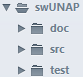
\includegraphics{unap_dir.png}}
\caption{swUNAP根目录组成}
\label{fig:unap_dir}
\end{figure}

\begin{figure}[htbp]
\centerline{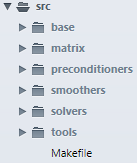
\includegraphics{src_dir.png}}
\caption{src目录组成}
\label{fig:src_dir}
\end{figure}

UNAP的根目录如图~\ref{fig:unap_dir}所示。doc文件夹包含了说明文档,src文件夹包含UNAP的主体代码模块,test文件夹则包含了一些测试算例和数据。src目录结构如图~\ref{fig:src_dir}所示:base包含了基本的宏、向量操作、MPI函数和指向多重对象的PtrList。matrix文件夹包含了关于矩阵结构的定义和操作,如LDU、CSR类型矩阵,矩阵的特征值求解、矩阵在AMG的粗化等。preconditioner文件夹包含了在Krylov子空间法中常用的几类预条件子:DIC(求解对称矩阵),DILU(求解非对称矩阵),diagonal(Jacobi类型迭代)和MG(多重网格预条件子,还未完善)。smoothers文件夹主要包含了在MG中用到的两类光滑器:Gauss-Seidel和Chebyshev。solvers文件夹下主要包含了前述的几种求解器(PCG,PBiCGStab和AMG)。tools文件夹下包含了一些工具,包括矩阵格式的转换(coo、csr和ldu之间的转换,完成了部分),ldu类型矩阵的打印输出,从Hypre或OpenFOAM打印输出矩阵的读取,计时函数、从核代码和与fortran的接口等。


\section{主要代数求解器使用说明}
在用户程序中使用UNAP的求解器主要步骤是:

\begin{enumerate}[label=\arabic*)]
\item 创建矩阵对象,需要的信息有:行数,对角线系数,上三角系数及对应的行、列号,上三角系数的个数,下三角系数(若与上三角系数不一样)
\item 创建求解器对象及对应的需要的组件对象(如CG法中的preconditioner,MG法中粗层网格算子),后面会分别说明
\item 选择控制参数
\item 调用solver的solve函数求解
\end{enumerate}

然后编译可执行程序,并链接libswunap.a(sw) 或 libunap.so(x86)。\\
下面举例说明(可参见test/ex11.cpp)

\subsection{PCG和PBiCGStab}
这两类方法都属于Krylov子空间迭代法,其中PCG用来求解对称方程,PBiCGStab用来求解对称、不对称方程。
\vspace{5mm}
\lstinputlisting{CG-example.cpp}
\vspace{3mm}

\subsection{AMG}
可用于求解对称、不对称方程,但对称方程会用到最快梯度下降法,收敛速度比不对称的要快。
\vspace{5mm}
\lstinputlisting{MG-example.cpp}
\vspace{3mm}


\section{编译说明}
目前版本支持x86和sw下分别编译,通过在make时定义PLA=x86或PLA=sw来选择。sw版本又分别支持主核和从核版本,通过在makefile中控制“-DSW\_SLAVE”
来进行有条件编译。

\subsection{编译lib}
在根目录或src目录下执行make all

\subsection{编译测试算例}{\label{sec:test}}
在test目录下执行 ./swSub exName nProcs 或 ./x86Sub exName nProcs。exName是测试例子的名字,如要测试例子ex11.cpp,则exName=ex11,测试例子ex12f.f90,则exName=ex12f,注意fortran程序名字结尾带有f。nProcs是运行的进程数,每个算例可以运行的进程数请参看其对应的测试数据包含几个进程,如ex11.cpp中使用了exData/openfoam/cavity/20w目录下的数据,共有1、2、4、16个进程可供选择。

\subsection{一键编译}
在根目录下执行 ./swSub exName nProcs 或 ./x86Sub exName nProcs,会同时编译lib文件。其他同~\ref{sec:test}。


\section{其它}

\end{document}
